\documentclass[border=10pt]{standalone}
\usepackage{tikz}
\usetikzlibrary{arrows.meta, calc}

\begin{document}
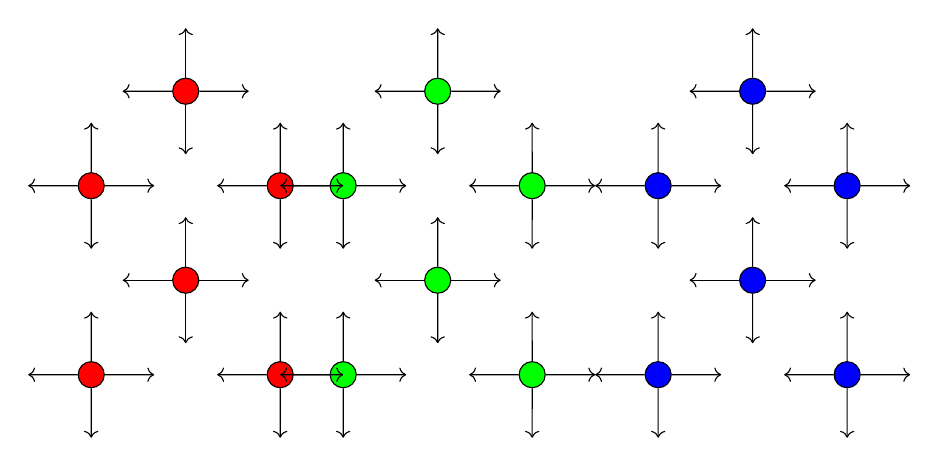
\begin{tikzpicture}[scale=0.8]
    % Red Subplot
    \node[draw, circle, fill=red] (r1) at (0, 3) {};
    \node[draw, circle, fill=red] (r2) at (-1.5, 1.5) {};
    \node[draw, circle, fill=red] (r3) at (1.5, 1.5) {};
    \node[draw, circle, fill=red] (r4) at (0, 0) {};
    \node[draw, circle, fill=red] (r5) at (-1.5, -1.5) {};
    \node[draw, circle, fill=red] (r6) at (1.5, -1.5) {};
    
    % Green Subplot
    \node[draw, circle, fill=green] (g1) at (4, 3) {};
    \node[draw, circle, fill=green] (g2) at (2.5, 1.5) {};
    \node[draw, circle, fill=green] (g3) at (5.5, 1.5) {};
    \node[draw, circle, fill=green] (g4) at (4, 0) {};
    \node[draw, circle, fill=green] (g5) at (2.5, -1.5) {};
    \node[draw, circle, fill=green] (g6) at (5.5, -1.5) {};
    
    % Blue Subplot
    \node[draw, circle, fill=blue] (b1) at (9, 3) {};
    \node[draw, circle, fill=blue] (b2) at (7.5, 1.5) {};
    \node[draw, circle, fill=blue] (b3) at (10.5, 1.5) {};
    \node[draw, circle, fill=blue] (b4) at (9, 0) {};
    \node[draw, circle, fill=blue] (b5) at (7.5, -1.5) {};
    \node[draw, circle, fill=blue] (b6) at (10.5, -1.5) {};
    
    % Arrows and Lines
    \foreach \a in {r1,r2,r3,r4,r5,r6} {
        \draw[->] (\a) -- ++(0,-1);
        \draw[->] (\a) -- ++(-1,0);
        \draw[->] (\a) -- ++(1,0);
        \draw[->] (\a) -- ++(0,1);
    }
    
    \foreach \a in {g1,g2,g3,g4,g5,g6} {
        \draw[->] (\a) -- ++(0,-1);
        \draw[->] (\a) -- ++(-1,0);
        \draw[->] (\a) -- ++(1,0);
        \draw[->] (\a) -- ++(0,1);
    }
    
    \foreach \a in {b1,b2,b3,b4,b5,b6} {
        \draw[->] (\a) -- ++(0,-1);
        \draw[->] (\a) -- ++(-1,0);
        \draw[->] (\a) -- ++(1,0);
        \draw[->] (\a) -- ++(0,1);
    }
\end{tikzpicture}
\end{document}